%----------------------------------------------------------------------------
\appendix
%----------------------------------------------------------------------------
\chapter*{\fuggelek}\addcontentsline{toc}{chapter}{\fuggelek}
\setcounter{chapter}{\appendixnumber}
%\setcounter{equation}{0} % a fofejezet-szamlalo az angol ABC 6. betuje (F) lesz
\numberwithin{equation}{section}
\numberwithin{figure}{section}
\numberwithin{lstlisting}{section}
%\numberwithin{tabular}{section}

%----------------------------------------------------------------------------
\section{Pictures of Demonstrator railway system} \label{appendix:HWPictures}
%----------------------------------------------------------------------------
%\begin{figure}[!h]
%	\centering
%	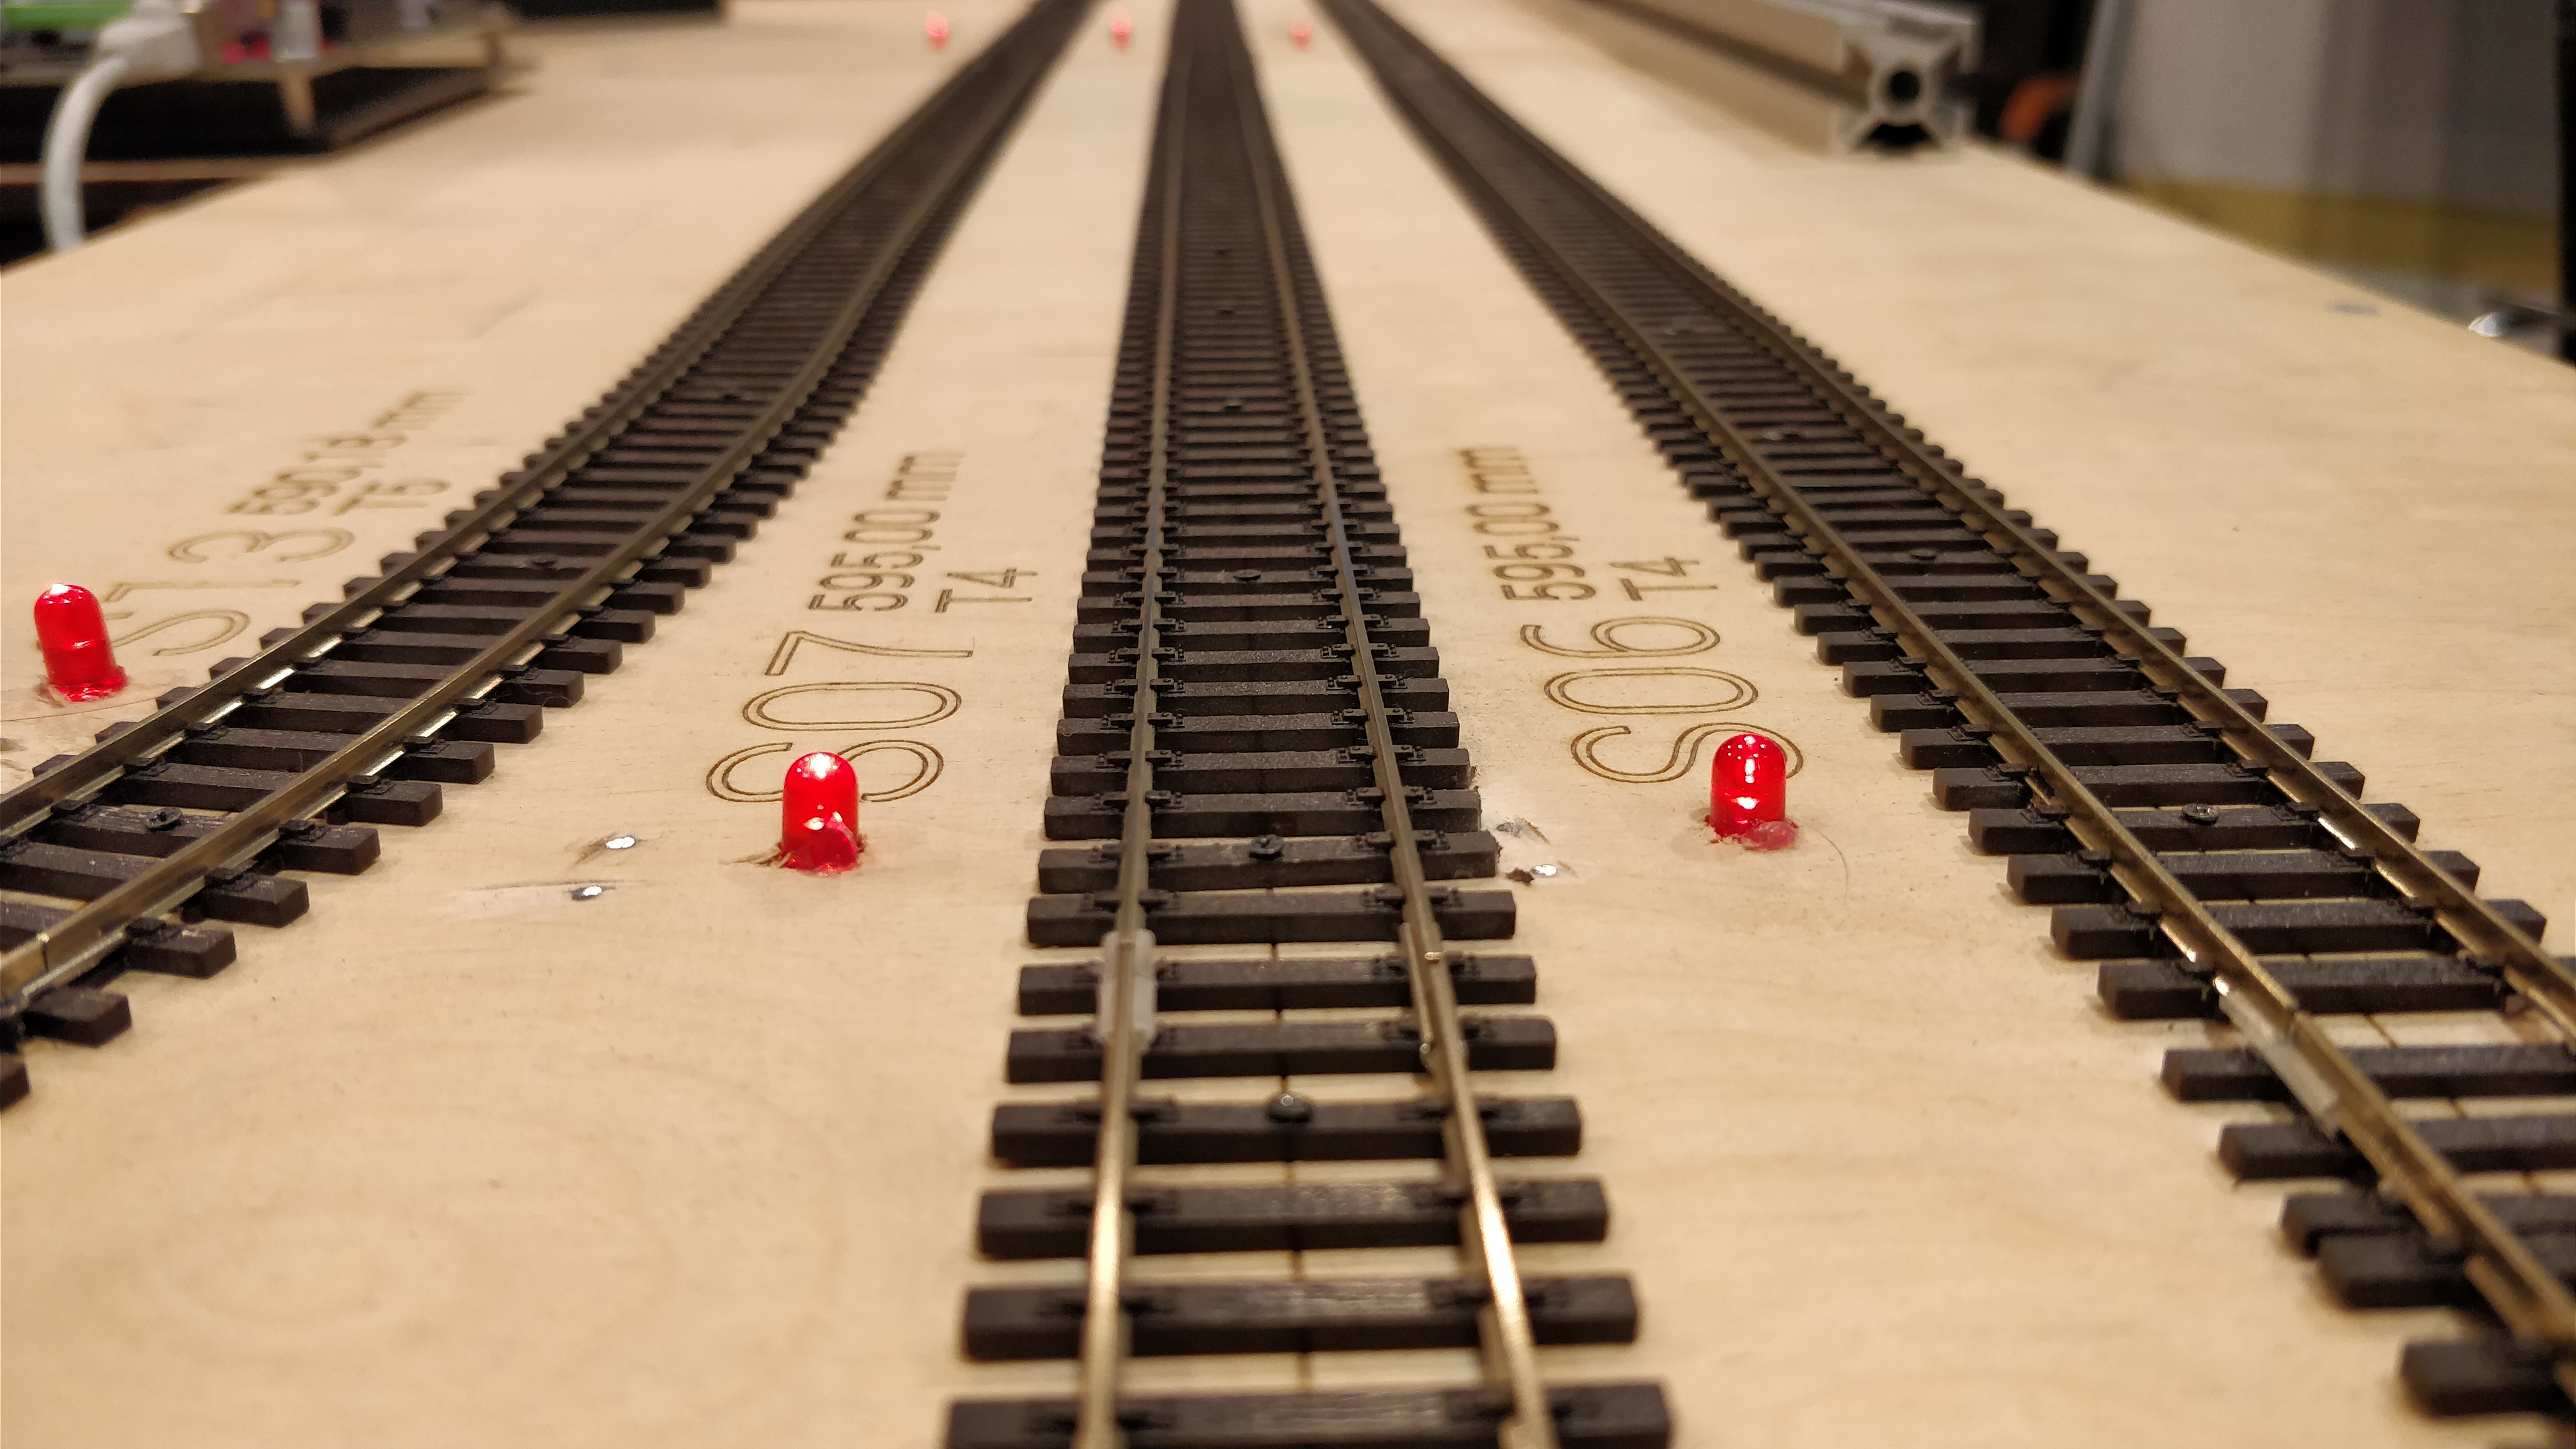
\includegraphics[width=150mm, keepaspectratio]{figures/modes3/section.jpg}
%	\caption{Railway Section}
%	\label{fig:section}
%\end{figure}
%
%\begin{figure}[!h]
%	\centering
%	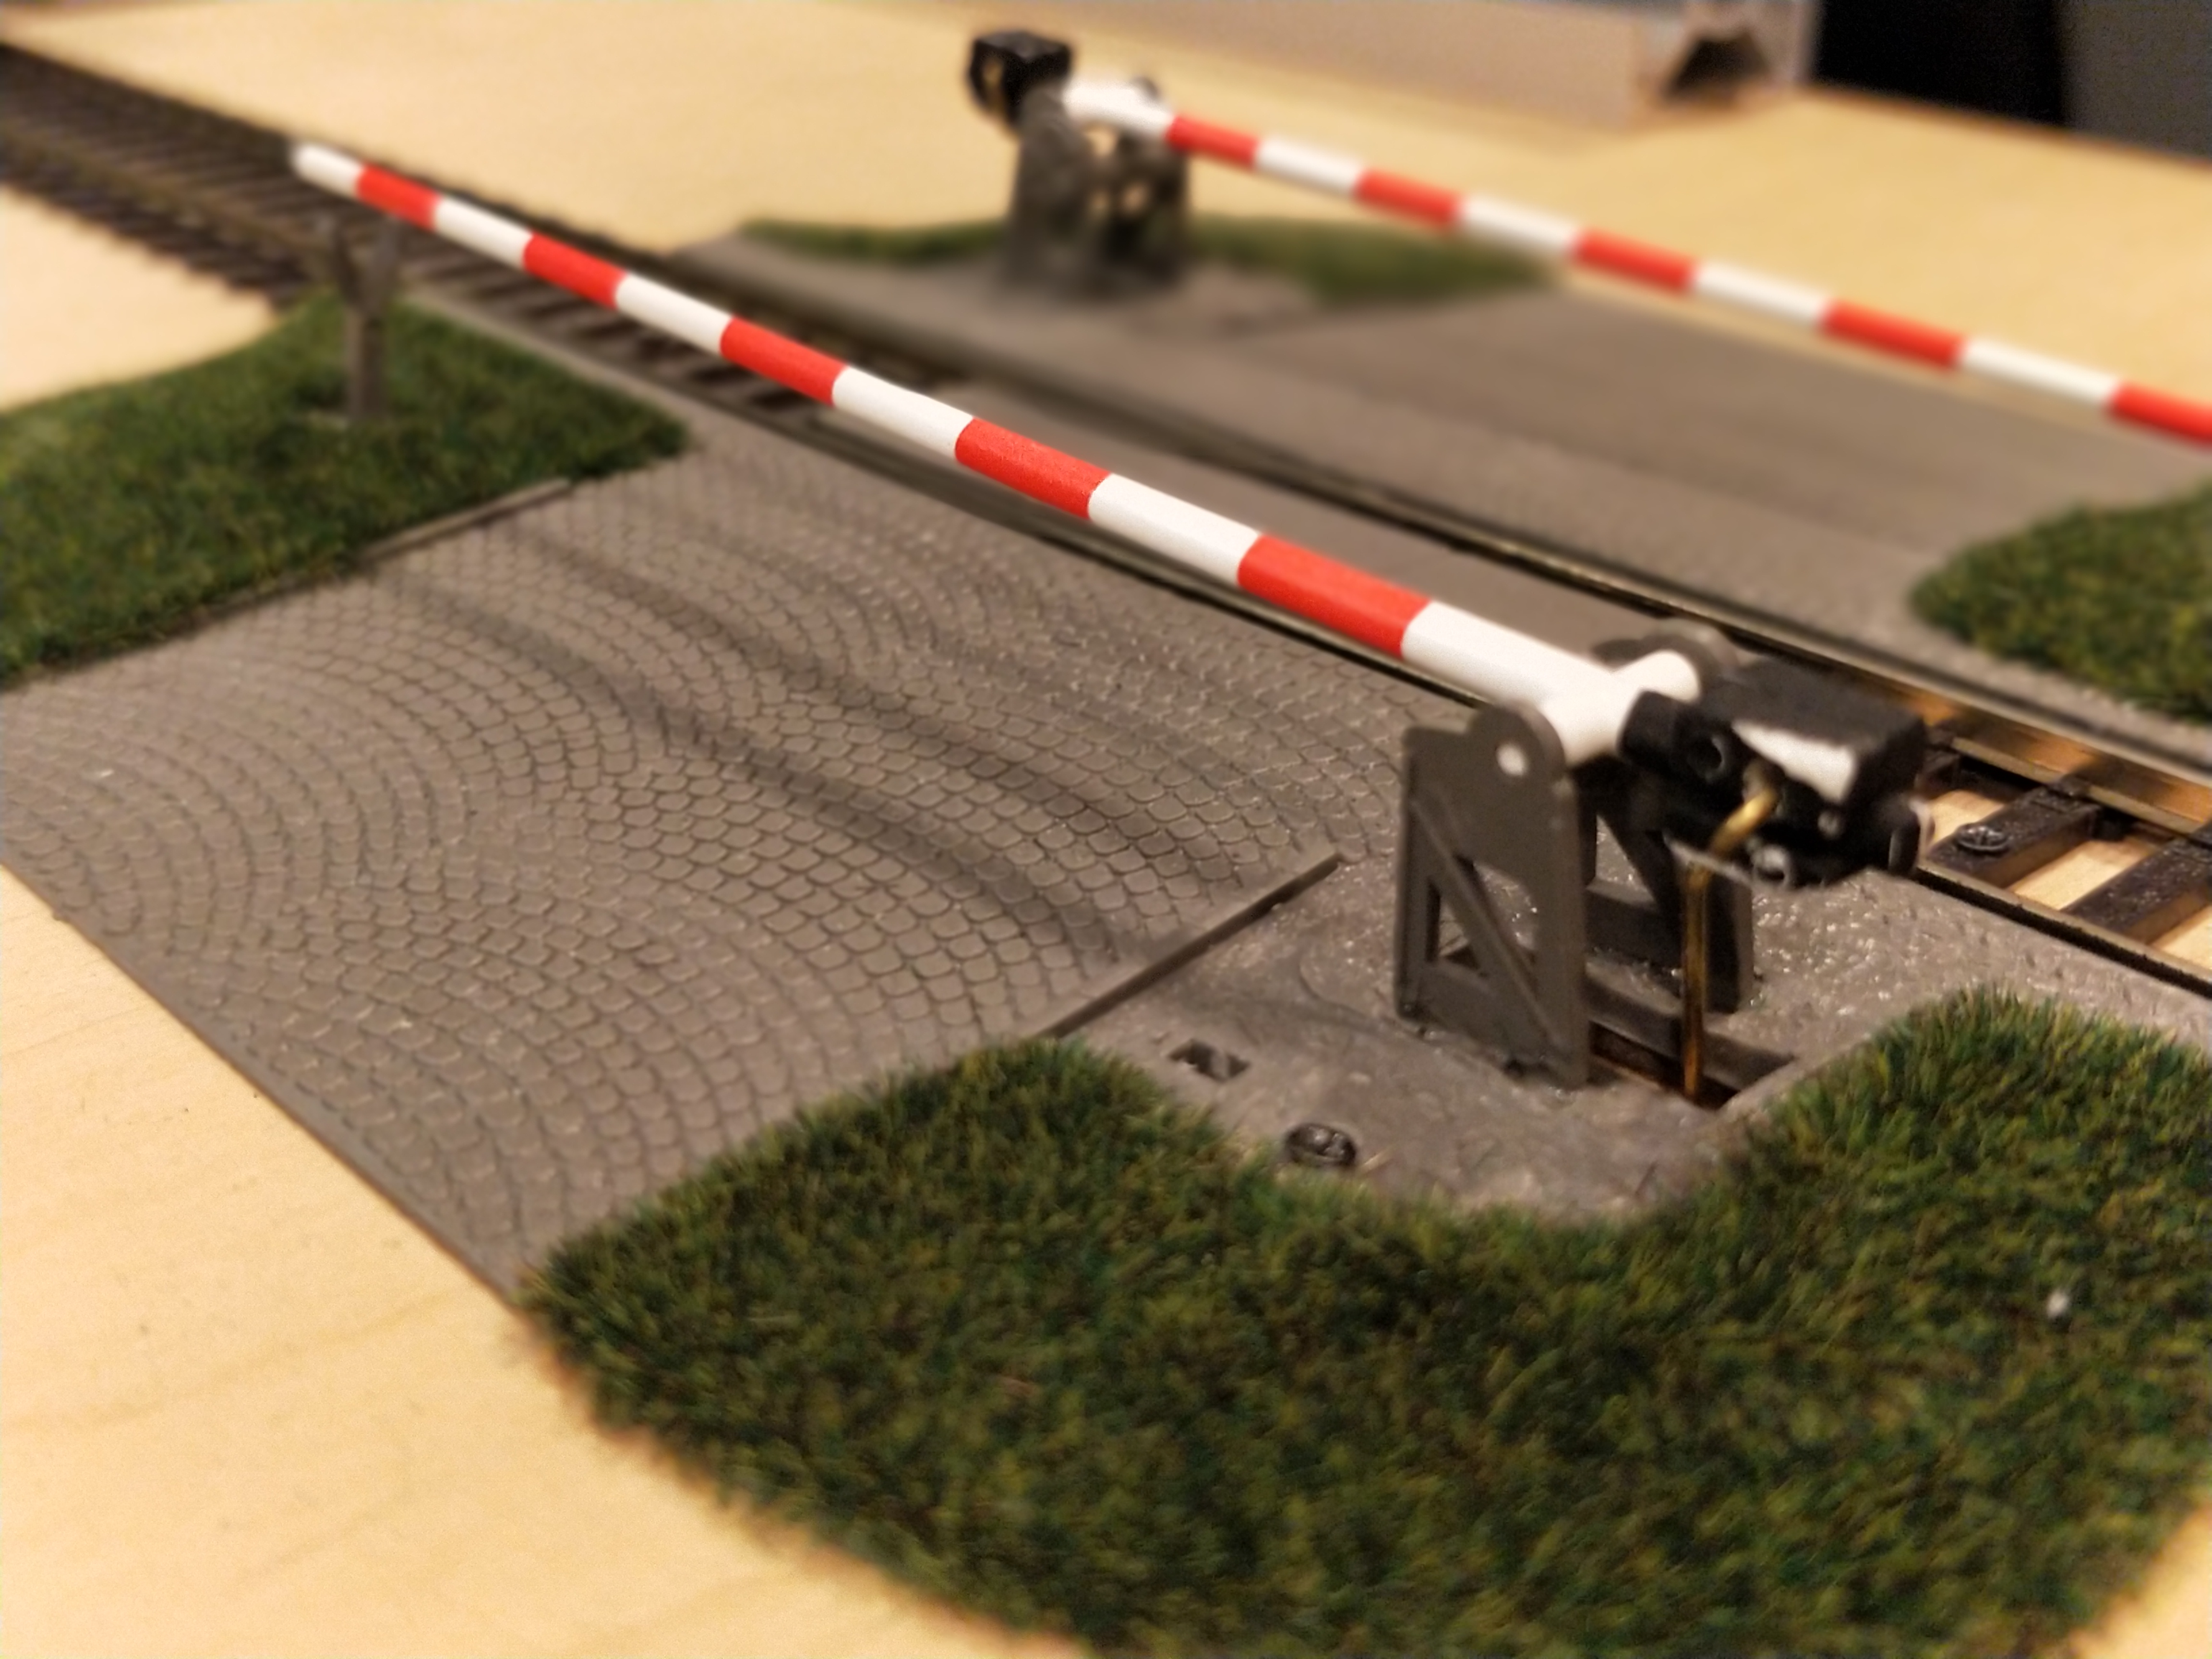
\includegraphics[width=150mm, keepaspectratio]{figures/modes3/barrier.jpg}
%	\caption{Barrier and passageway}
%	\label{fig:barrier}
%\end{figure}
%
%
%\begin{figure}[!h]
%	\centering
%	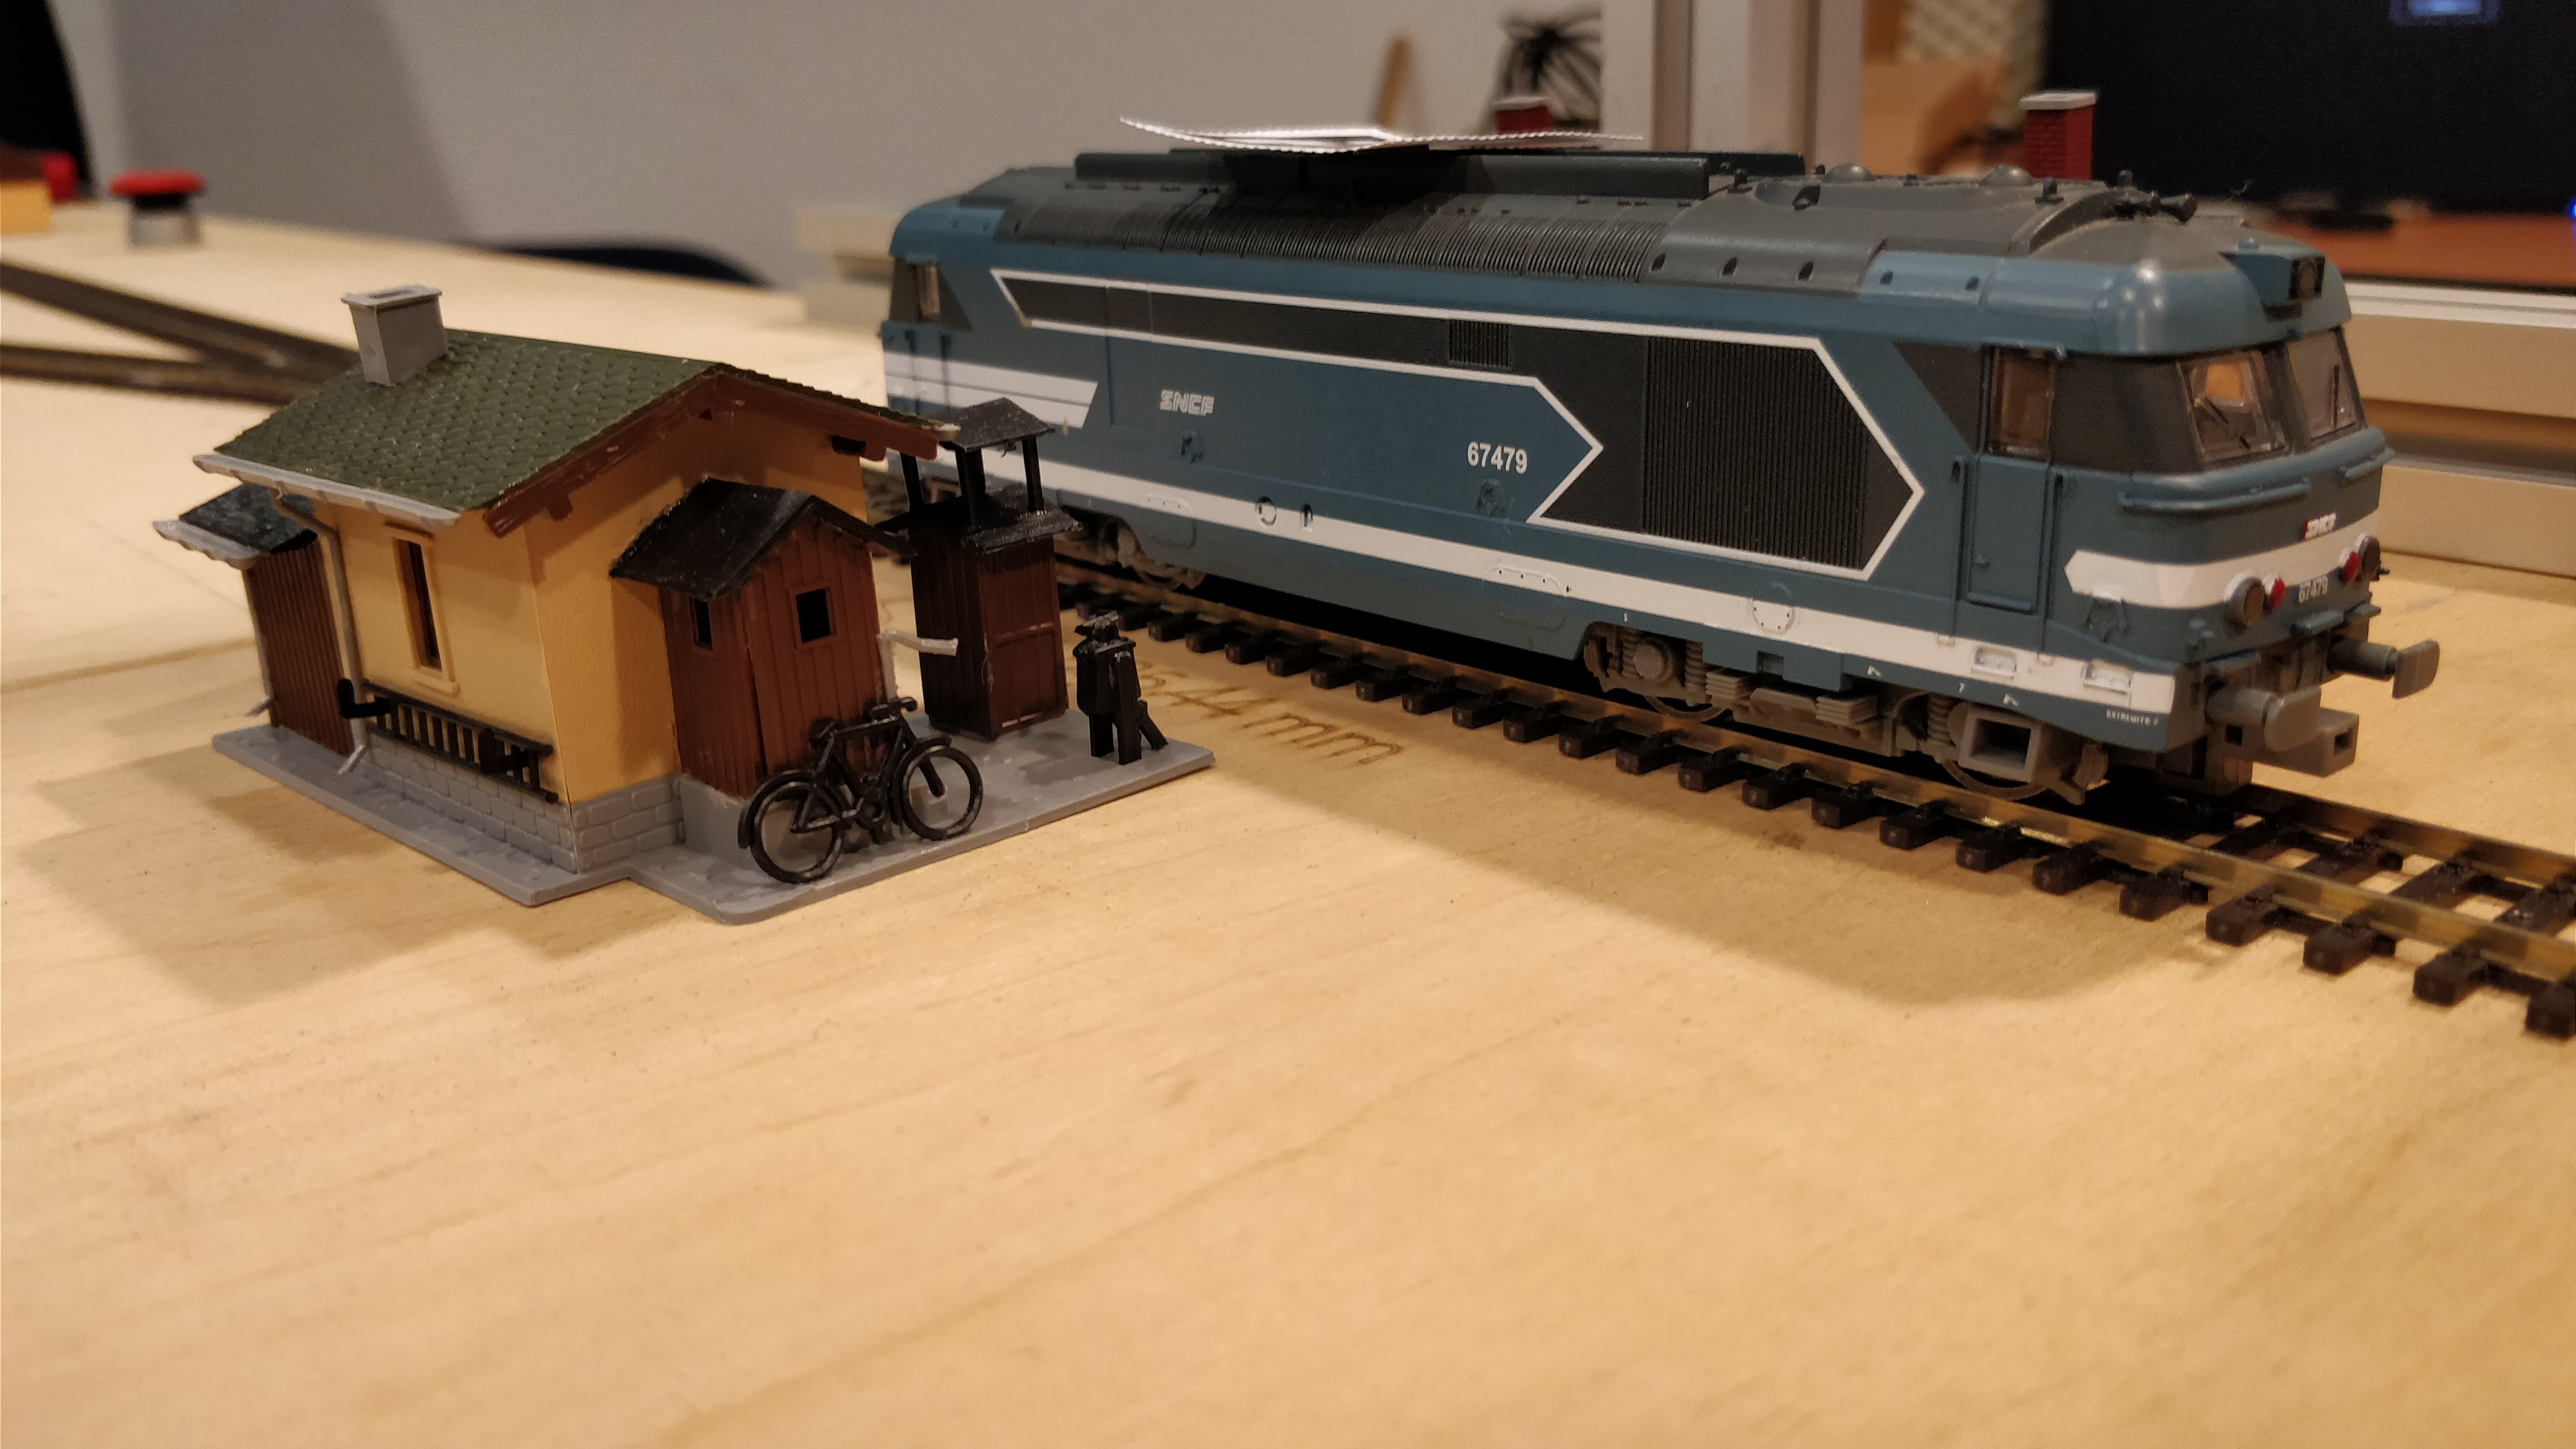
\includegraphics[width=150mm]{figures/modes3/train.jpg}
%	\caption{Train}
%	\label{fig:train}
%\end{figure}
%
%\begin{figure}[!h]
%	\centering
%	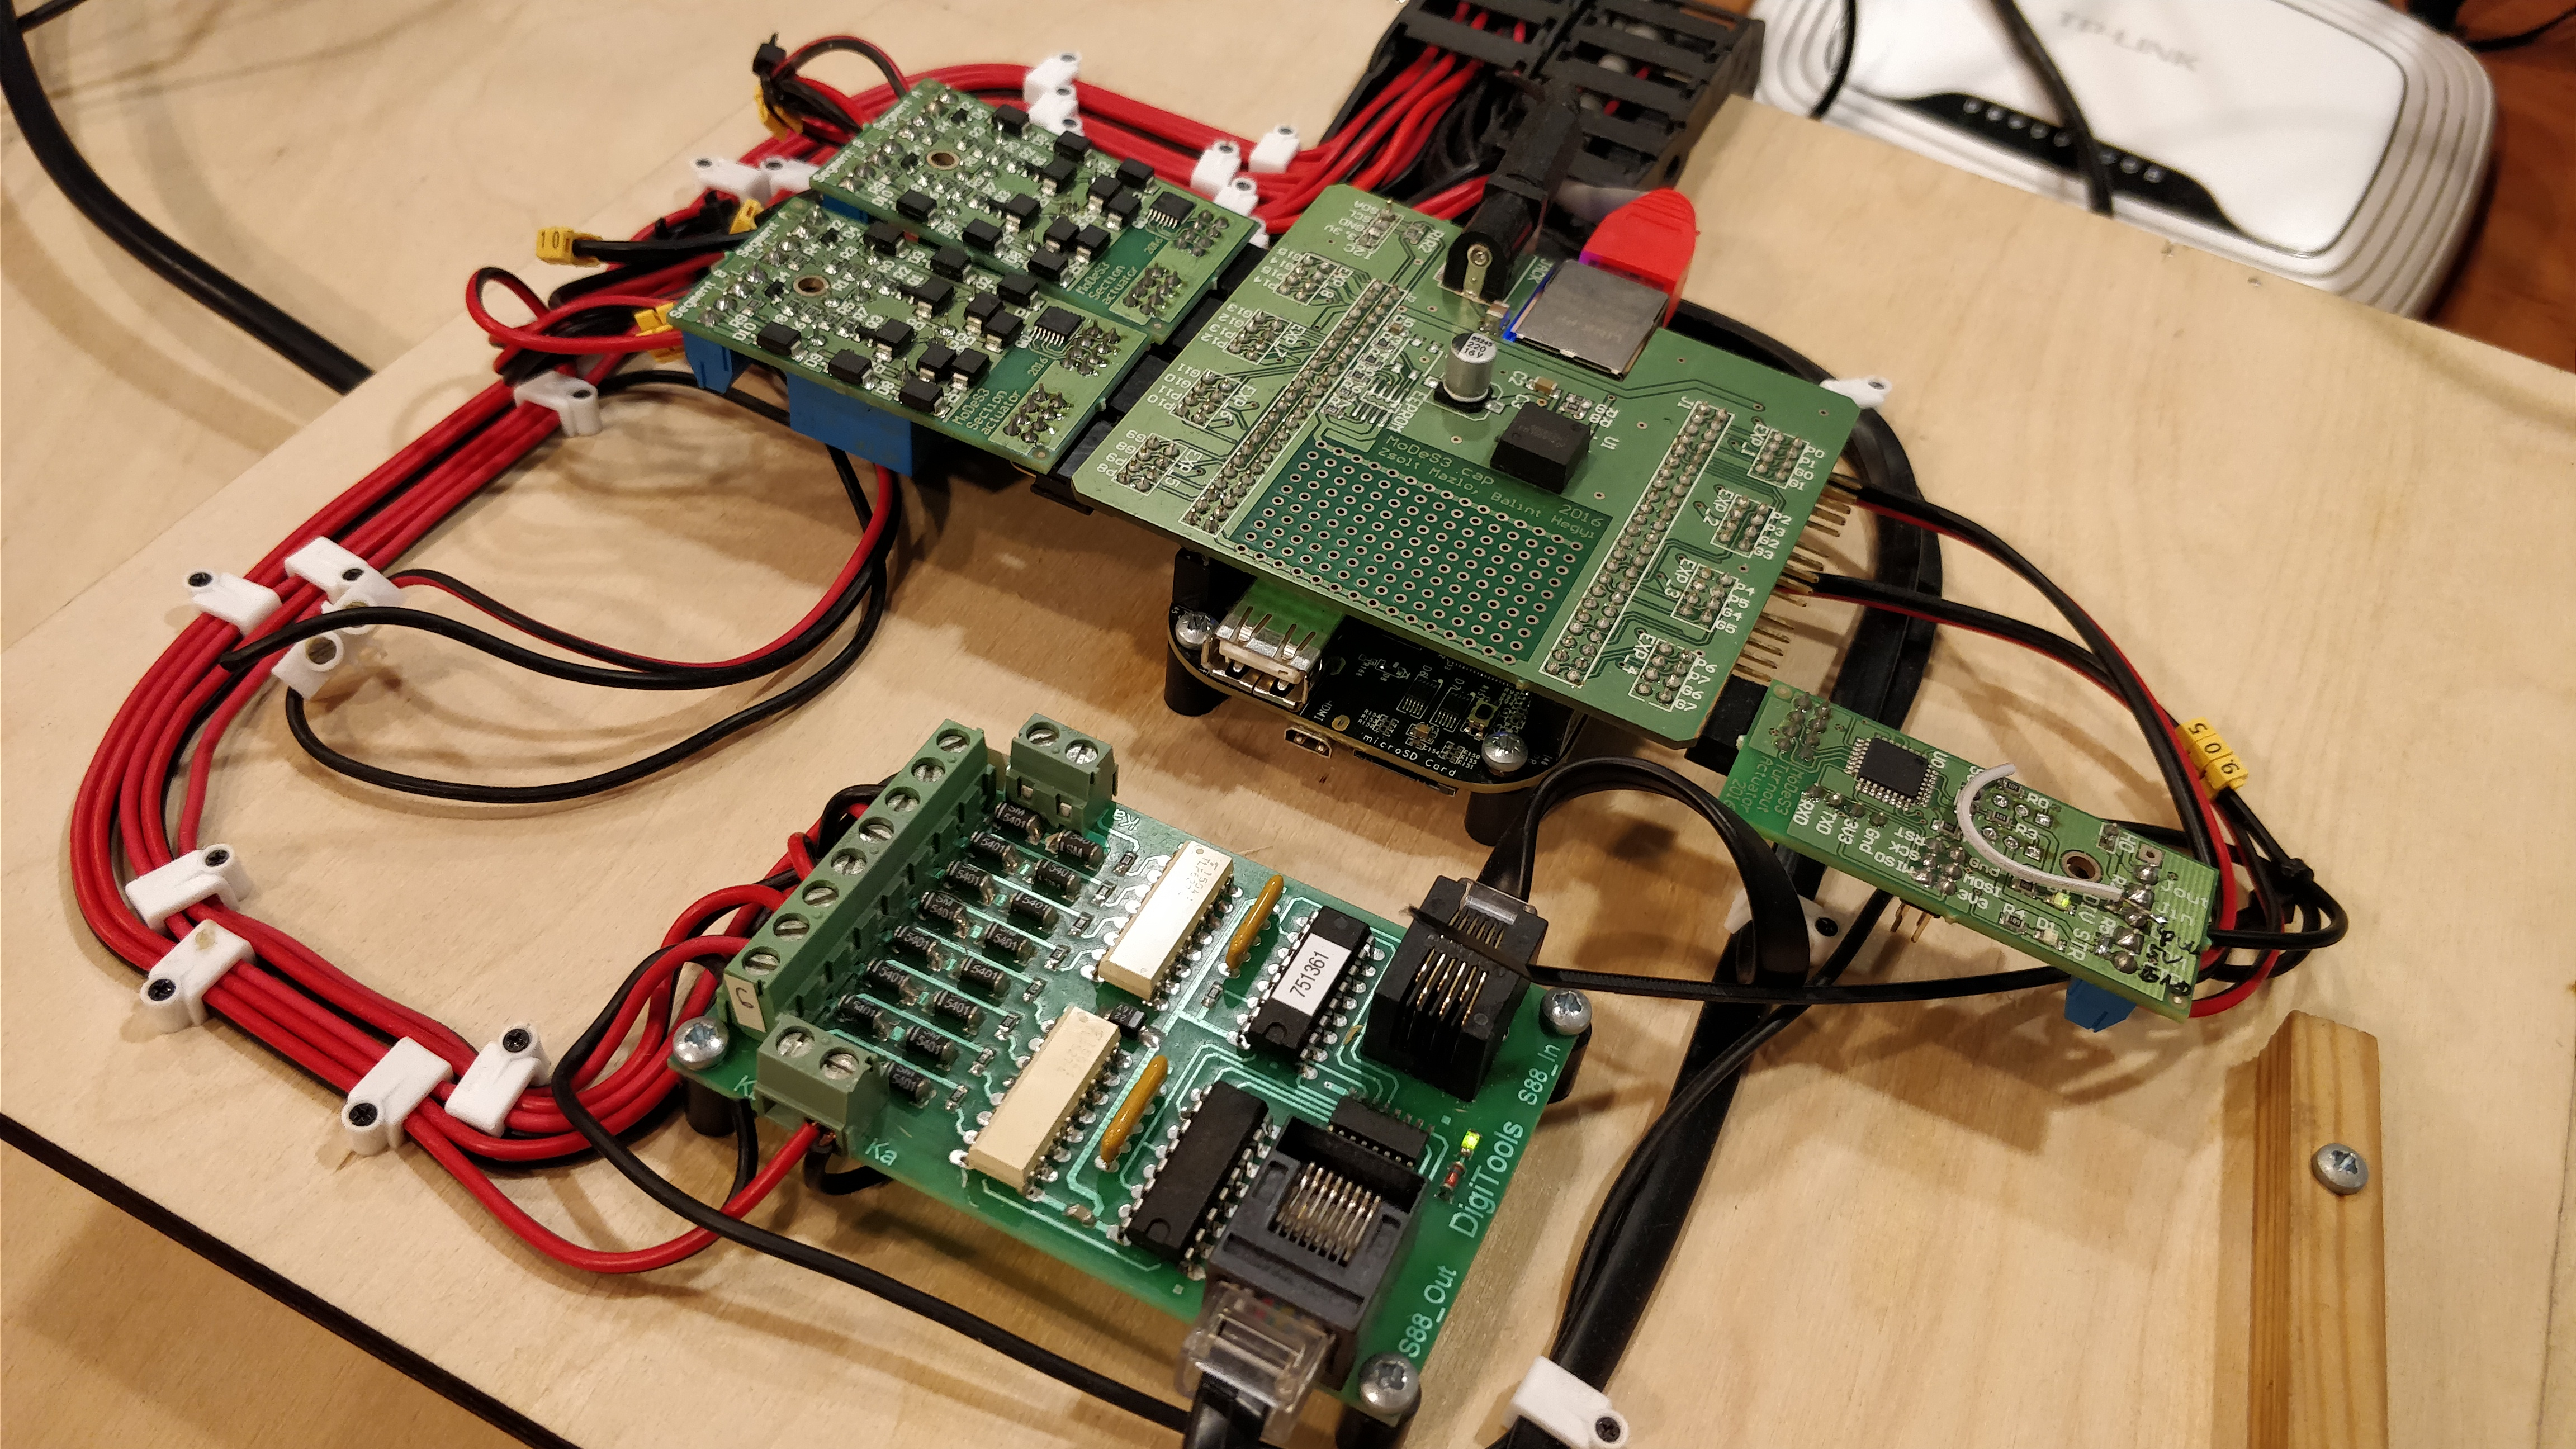
\includegraphics[width=150mm]{figures/modes3/segmentControlling.jpg}
%	\caption{Cape, segment and turnout actuator attached to BBB and connection to segment sensor}
%	\label{fig:BBBinAll}
%\end{figure}
%
%\begin{figure}[!h]
%	\centering
%	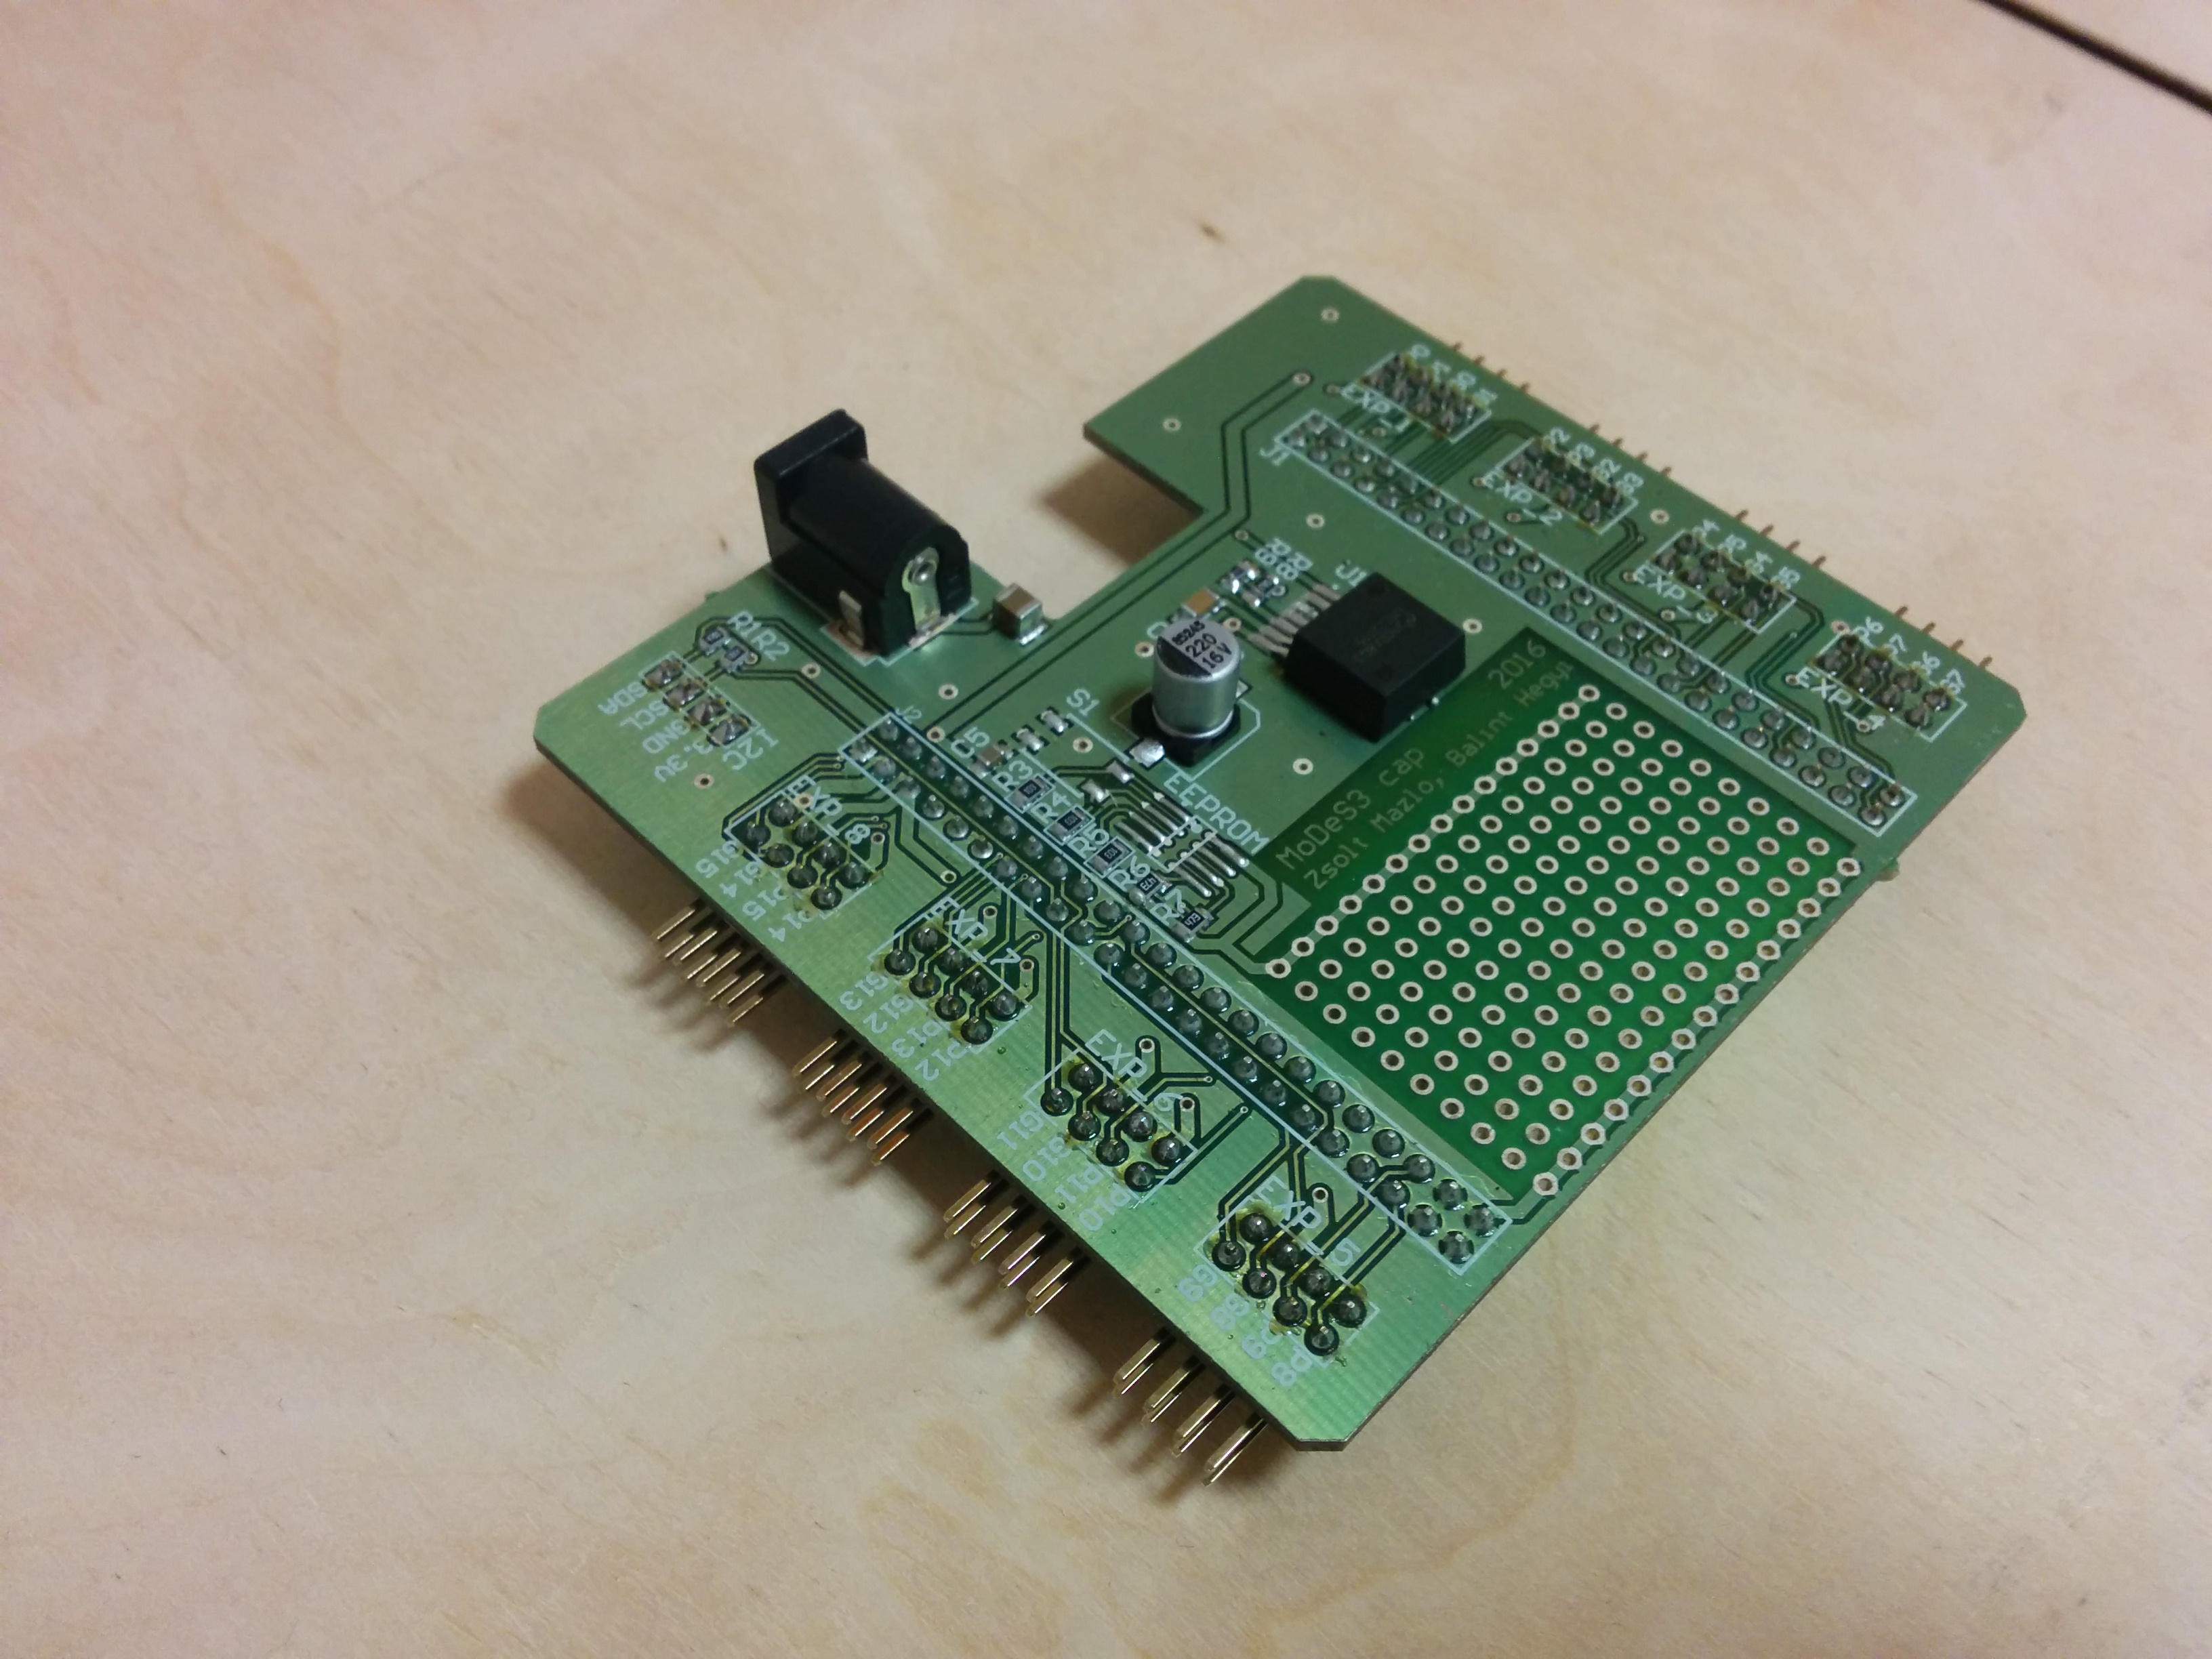
\includegraphics[width=100mm]{figures/modes3/cap1.jpg}
%	\caption{Cape and expander for BeagleBone Black}
%	\label{fig:cape}
%\end{figure}
%
%\begin{figure}[!h]
%	\centering
%	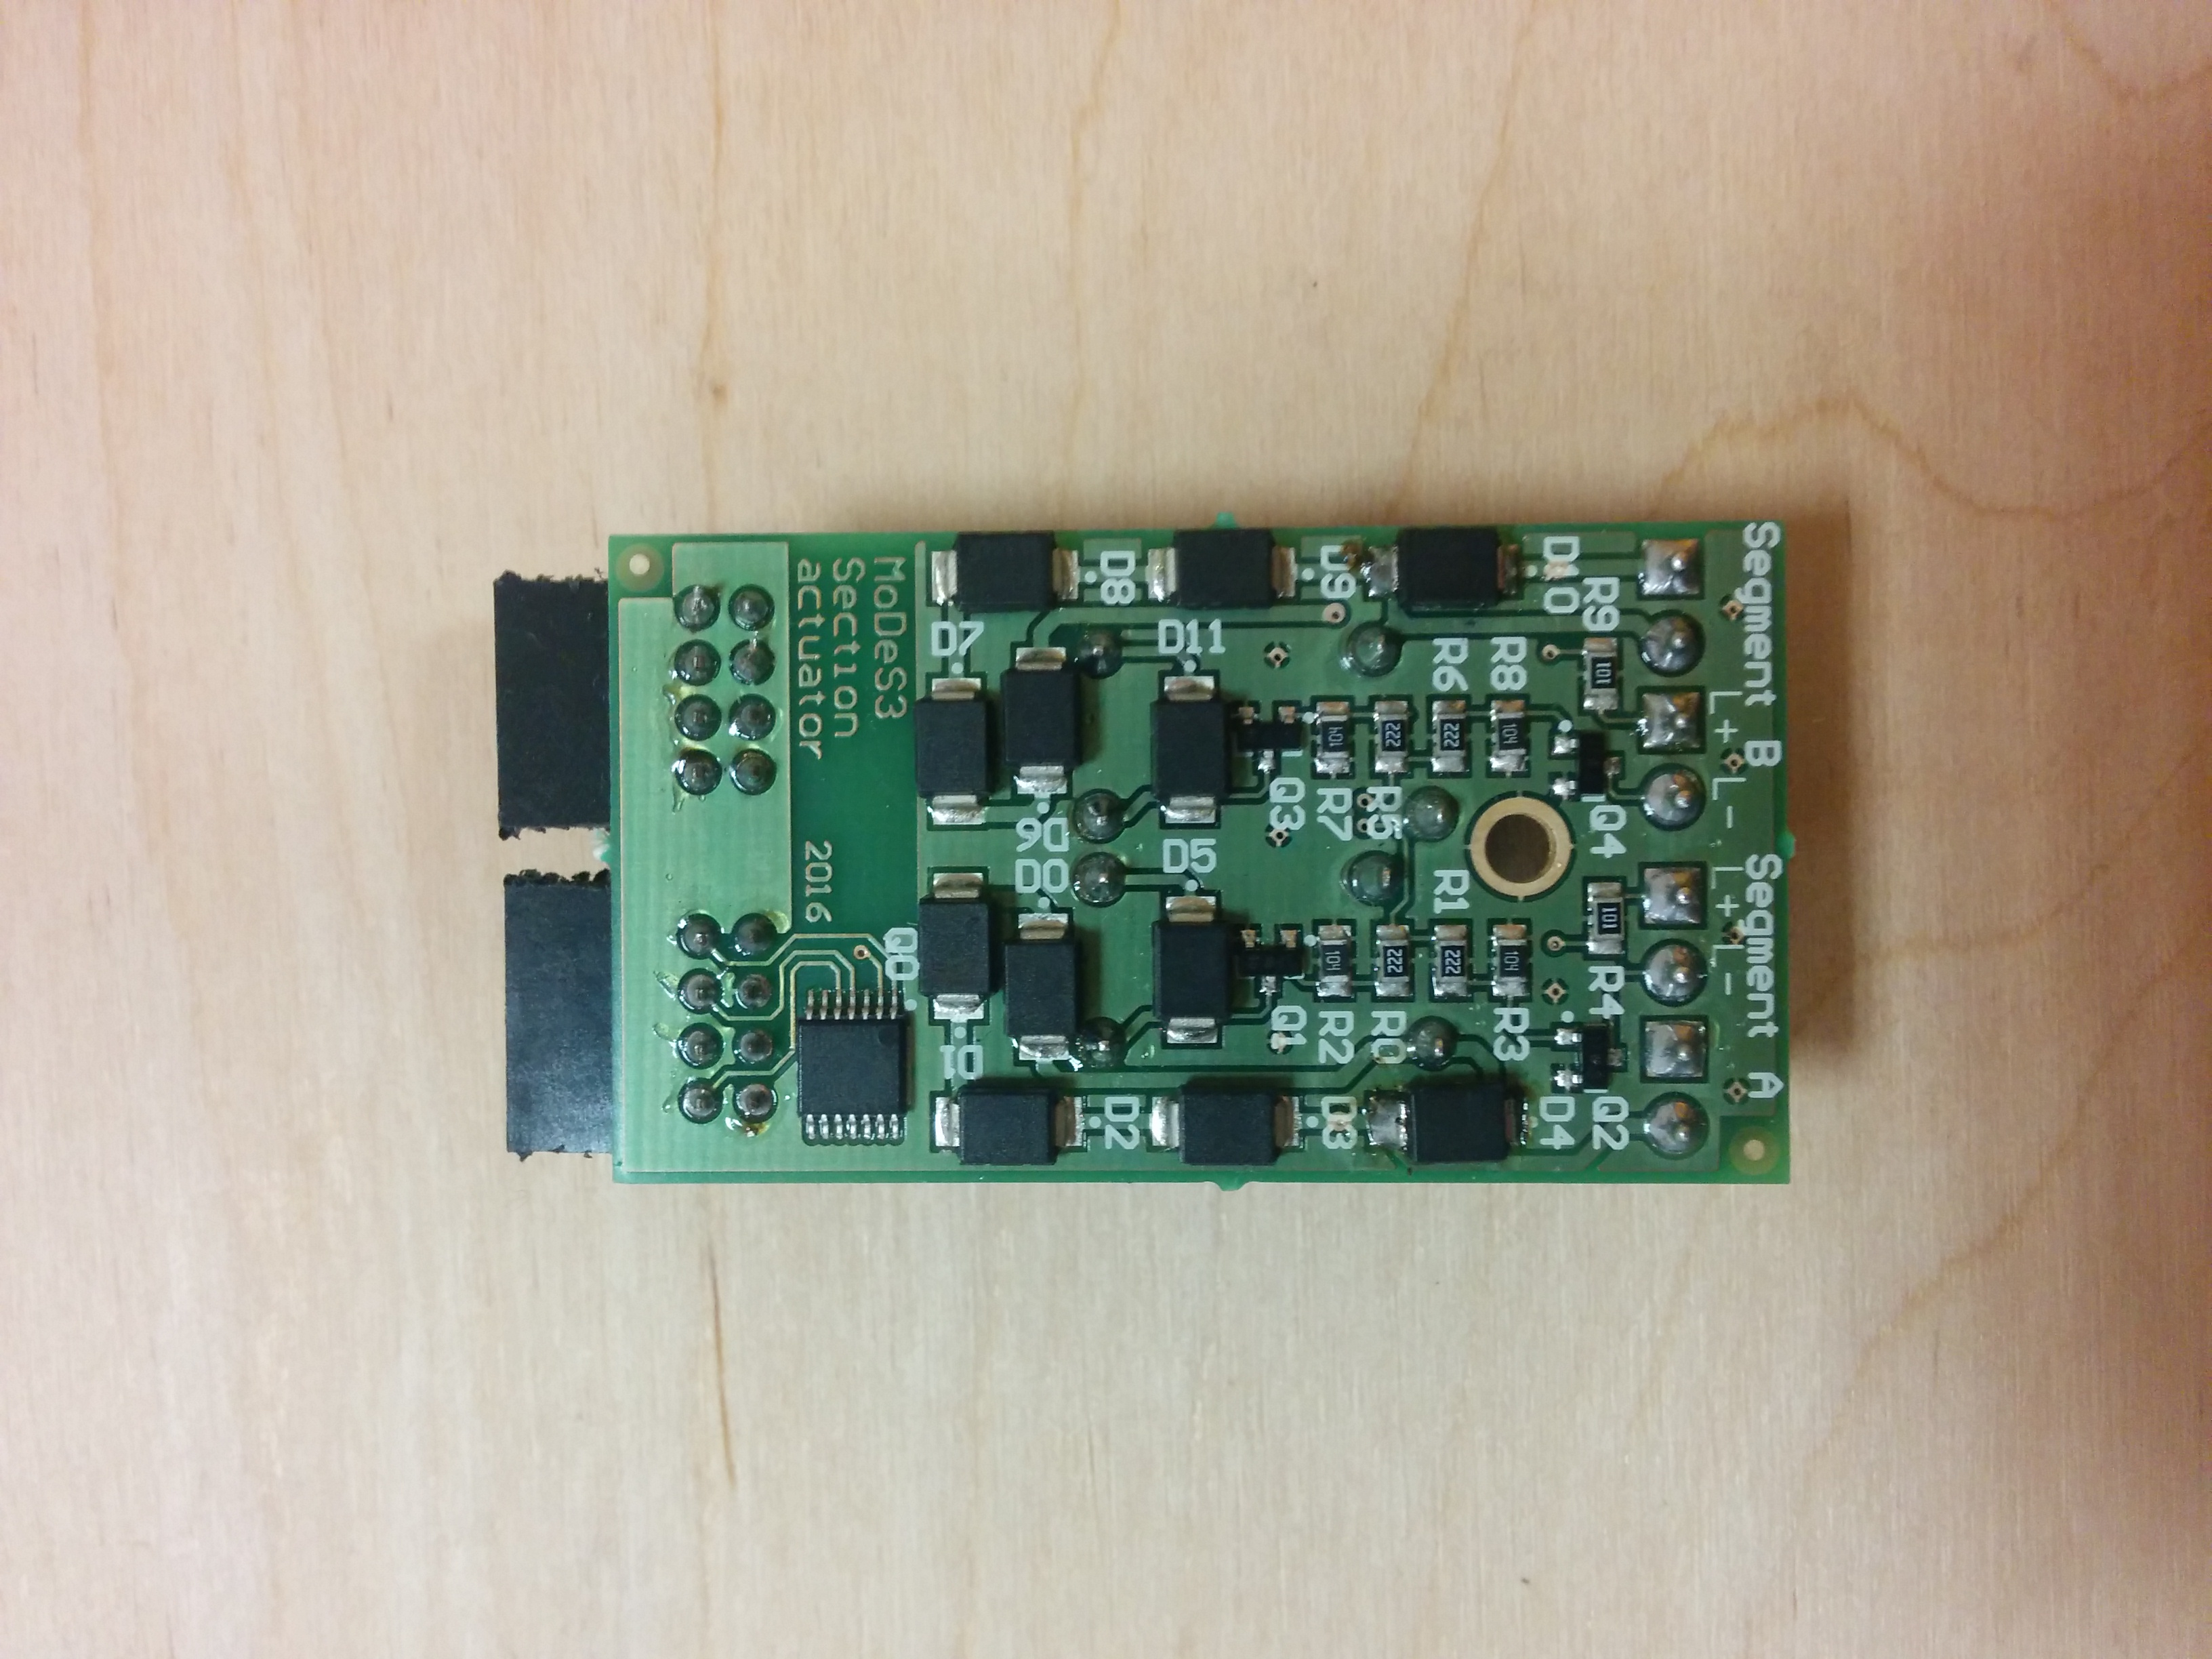
\includegraphics[width=100mm]{figures/modes3/segment-top.jpg}
%	\caption{Segment actuator top view}
%	\label{fig:segmentTop}
%\end{figure}
%
%\begin{figure}[!h]
%	\centering
%	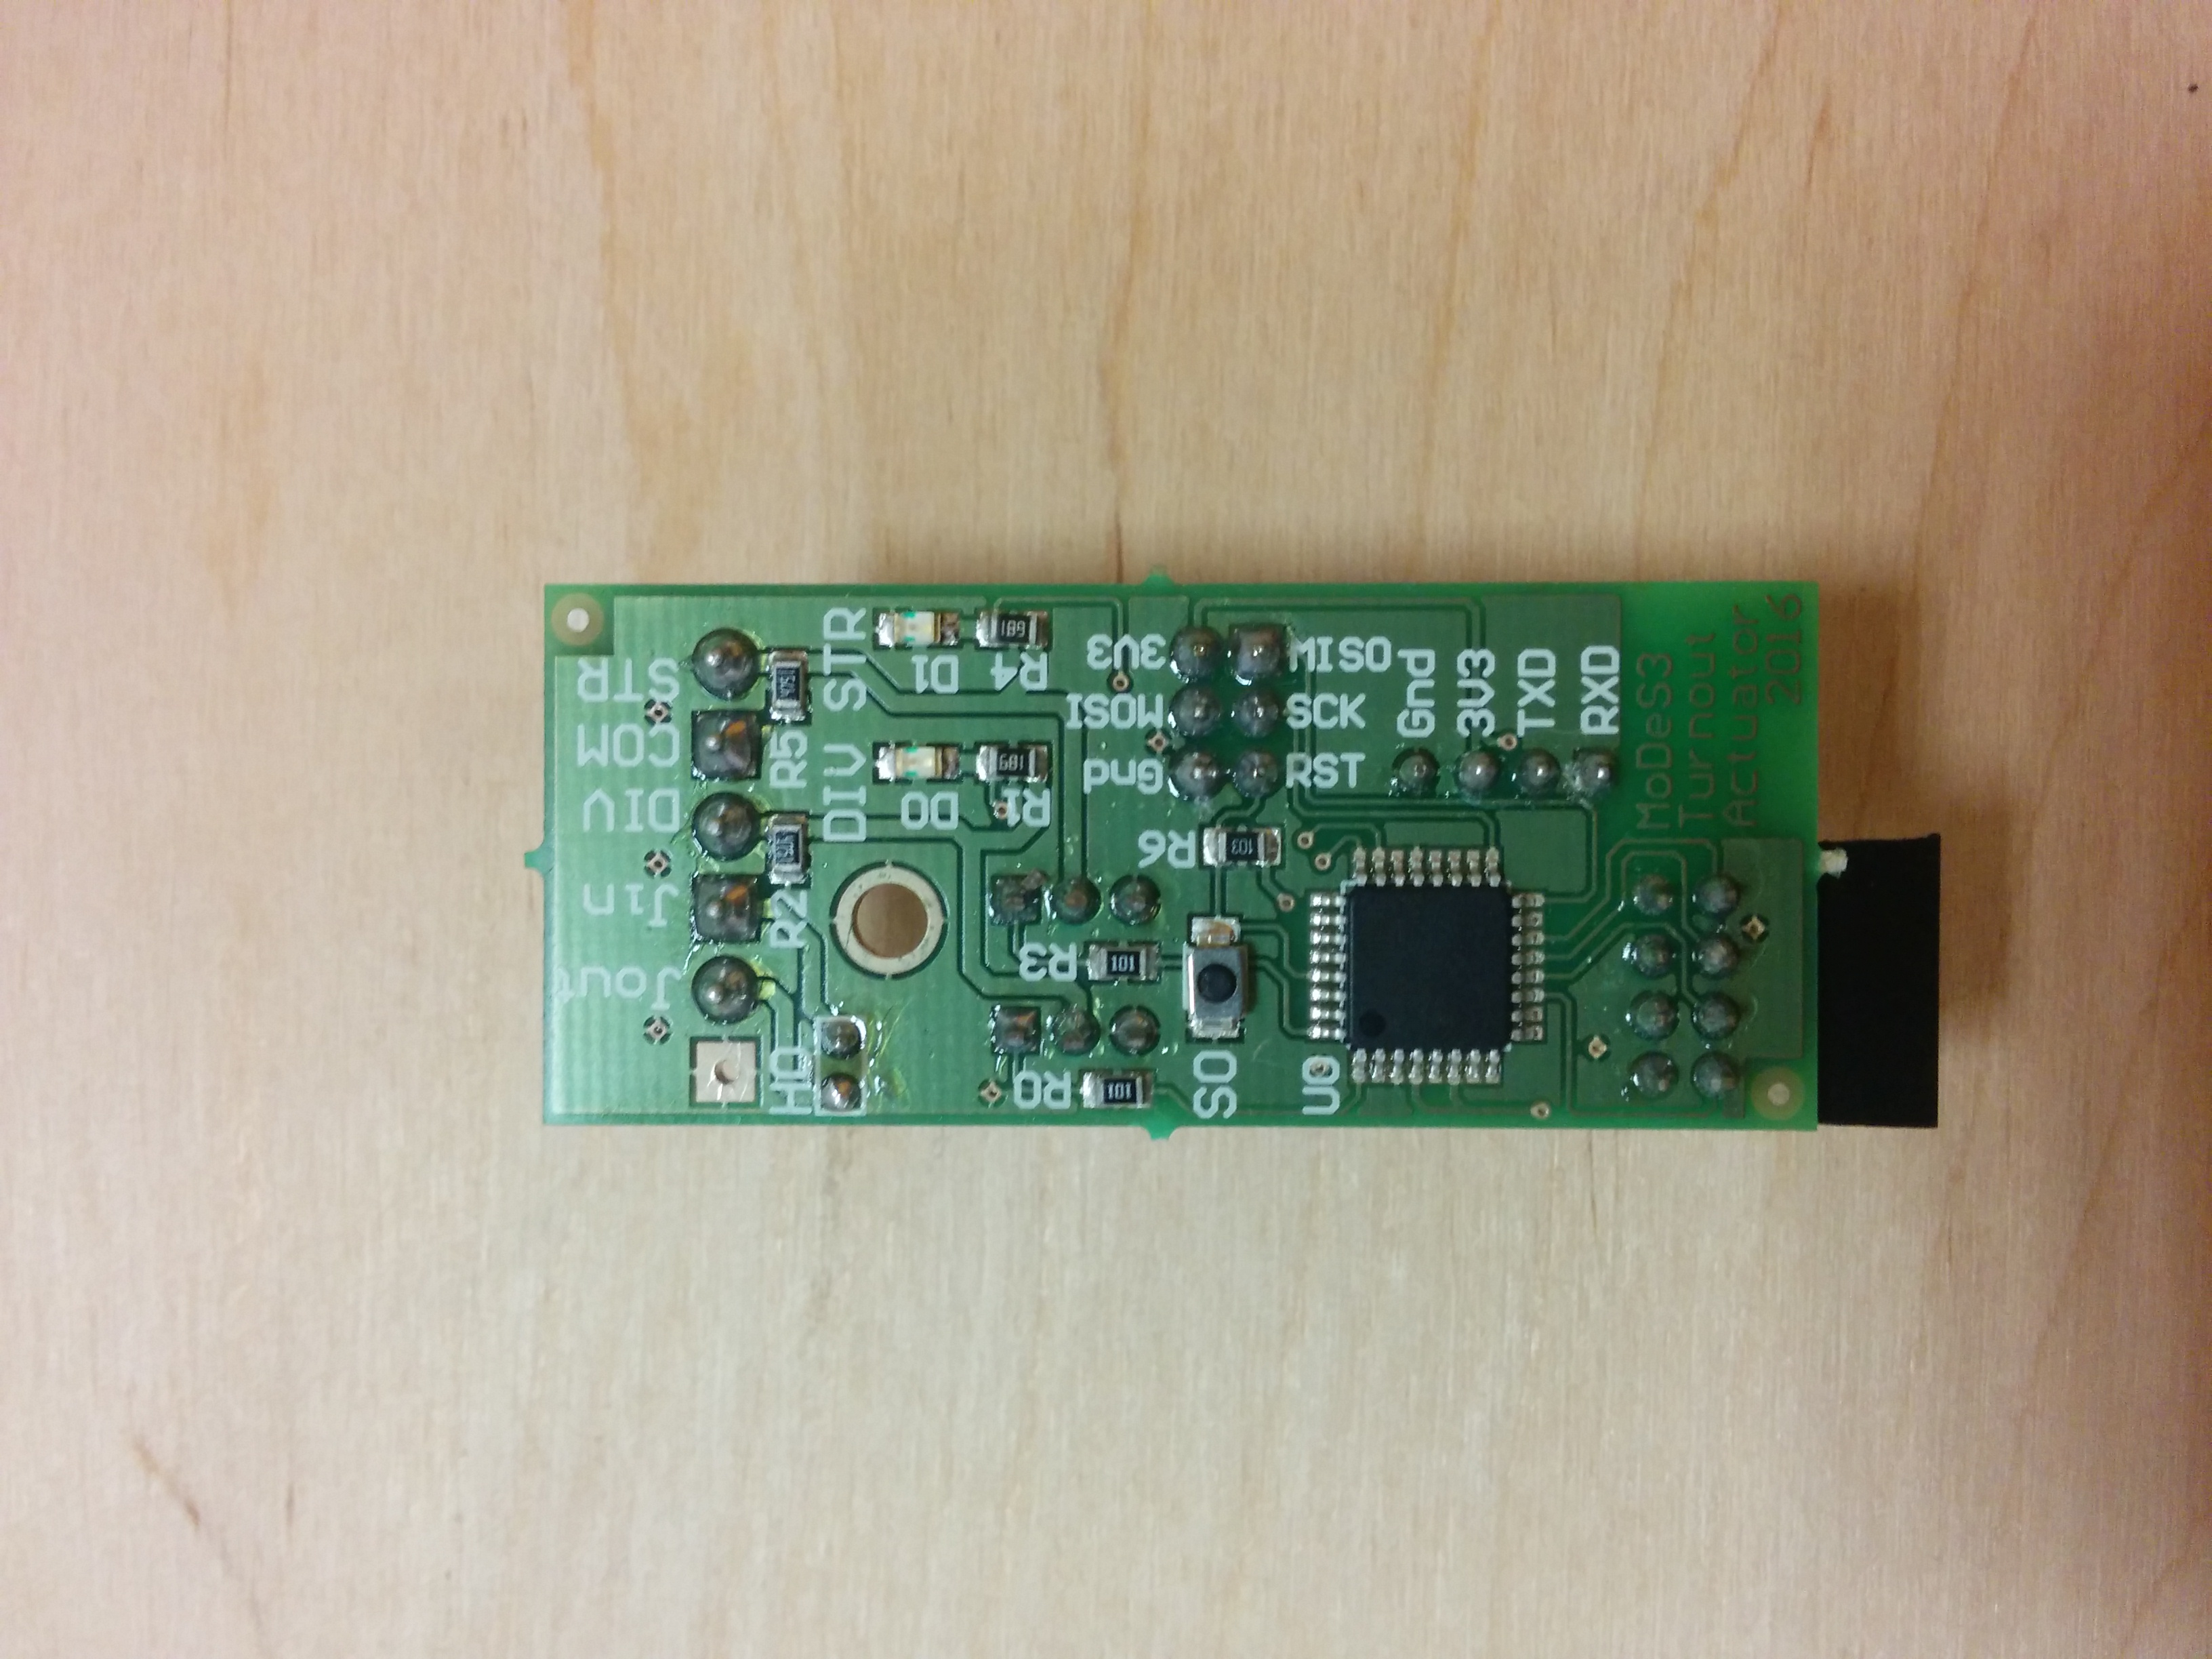
\includegraphics[width=100mm]{figures/modes3/turnout-top.jpg}
%	\caption{Turnout actuator top view}
%	\label{fig:turnoutTop}
%\end{figure}

